\documentclass[11pt]{article}
\usepackage[a4paper,margin=0.92in]{geometry}
\usepackage{amsmath,amssymb,amsthm,mathtools}
\usepackage{booktabs,array,graphicx,xcolor,xurl}
\usepackage[hidelinks]{hyperref}
\hypersetup{pdftitle={Exact Memory of Finite Spectral Routing Tables},pdfauthor={Lluis Eriksson},pdfsubject={Direct-sum occupancy law for passive spectral routing}}
\usepackage[nameinlink,capitalise]{cleveref}
\usepackage{microtype,etoolbox}
\AtBeginEnvironment{thebibliography}{\fontsize{8}{9}\selectfont\setlength{\itemsep}{-2pt}\setlength{\parsep}{0pt}}

\newtheorem{theorem}{Theorem}[section]
\newtheorem{lemma}[theorem]{Lemma}
\newtheorem{corollary}[theorem]{Corollary}
\newtheorem{proposition}[theorem]{Proposition}
\theoremstyle{definition}\newtheorem{definition}[theorem]{Definition}\newtheorem{example}[theorem]{Example}
\theoremstyle{remark}\newtheorem{remark}[theorem]{Remark}\newtheorem{limitation}[theorem]{Limitation}
\crefname{lemma}{Lemma}{Lemmas}\crefname{proposition}{Proposition}{Propositions}
\crefname{corollary}{Corollary}{Corollaries}\crefname{limitation}{Limitation}{Limitations}
\newcommand{\C}{\mathbb C}\newcommand{\D}{\mathbb D}\newcommand{\T}{\mathbb T}
\newcommand{\ran}{\operatorname{ran}}\newcommand{\Span}{\operatorname{span}}
\newcommand{\rank}{\operatorname{rank}}
\newcommand{\mcdeg}{\deg_{\mathrm{McM}}}\newcommand{\A}{\mathcal A}
\newcommand{\norm}[1]{\lVert#1\rVert}\newcommand{\dd}{\,\mathrm d}
\newcolumntype{L}[1]{>{\raggedright\arraybackslash}p{#1}}

\title{Exact Memory of Finite Spectral Routing Tables:\\
The Direct-Sum Occupancy Law and Its Singular Strata}
\author{Lluis Eriksson}
\date{11 August 2026}

\begin{document}
\maketitle

\begin{abstract}
We give a single exact state-counting theory for finite passive spectral
routing tables.  Fix distinct boundary frequencies, one input $k$-plane,
and a word $w$ whose symbol $a$ requests a target $k$-plane $Y_a$ exactly
$n_a$ times.  If the used targets are in direct-sum position---they need not
be orthogonal and may have arbitrarily small principal angles---then the
minimum McMillan degree among square finite rational-inner interpolants is
\[
             d_{\min}=k\bigl(L-\min_a n_a\bigr).
\]
Thus the rarest target fixes generic passive memory, independently of node
spacing and word order.

The lower bound uses block-dual detectors: direct-sum geometry supplies a
constant compression that is invertible on one target and annihilates every
other target.  Its determinant has $k$ forced zeros at every wrong node,
while a Blaschke--Potapov minor has no more zeros than the network has
states.  The upper bound is a matrix spectral compiler.  Target-weighted
node polynomials form a full-rank polynomial column; matrix
Fej\'er--Riesz factorization normalizes it to a rational-inner column of
degree at most the lower bound, and a degree-preserving lossless completion
closes the network.

The theorem strictly contains orthogonal fan-out, generic all-distinct
fan-out, and repeated orthogonal routing as special cases.  Beyond the
direct-sum locus we prove a detector-rank hierarchy: every constant
$k$-row detector contributes a weighted sum of its rank deficiencies to a
universal degree lower bound.  For lines this becomes a maximum weighted
hyperplane-occupancy bound and exactly resolves the complete three-line
phase diagram.  We also give a span sandwich, open-dense genericity,
fail-closed noisy certification, an exact collision discontinuity, and the
optimal integrated Wigner--Smith delay.  A producer and independent
verifiers audit 512 nonorthogonal scalar tables, 256 block tables, six
near-collision openings, and exact singular-incidence fixtures.  All source,
frozen evidence, and release metadata are linked visibly in the paper.
\end{abstract}

\noindent\textbf{Keywords:} rational inner matrix; McMillan degree;
subspace interpolation; Fej\'er--Riesz factorization; passive memory;
spectral routing; Wigner--Smith delay; collision strata.

\section{One table, three formerly separate regimes}

A finite lossless discrete-time network is represented by a square rational
matrix $S$, analytic on $\D$ and unitary almost everywhere on $\T$.  Its
McMillan degree is the state dimension of a minimal conservative
realization.  Let $\zeta_1,\ldots,\zeta_L\in\T$ be distinct, let
$X\subset\C^N$ be a $k$-plane, and let a word
$w=w_1\cdots w_L$ use the targets $Y_a\subset\C^N$.  We impose only
subspace data,
\begin{equation}\label{eq:task}
                         S(\zeta_i)X=Y_{w_i},\qquad 1\le i\le L,
\end{equation}
so bases and endpoint phases remain free.  Every competitor is square,
finite rational inner, and regular at the interpolation nodes.  Put
\[
 n_a=\#\{i:w_i=a\},\qquad n_*=\min_{a\in\A(w)}n_a,
 \qquad m=|\A(w)|.
\]

Earlier papers treated fully distinct orthogonal targets, fully distinct
direct-sum targets, and repeated orthogonal targets separately
\cite{ErikssonOrthogonal2026,ErikssonDirectSum2026,ErikssonRoutingWord2026}.
The missing intersection was the natural one: repeated targets with dense,
nonorthogonal Gram matrix.  That intersection produces the master law.

\begin{definition}[Direct-sum target table]\label{def:direct-sum}
The used targets are in direct-sum position if
\begin{equation}\label{eq:direct-sum}
               \dim\sum_{a\in\A(w)}Y_a=mk.
\end{equation}
Equivalently, for any isometric frames $W_a$ of $Y_a$, the block column
$W=[W_1\ \cdots\ W_m]$ has full column rank.
\end{definition}

\begin{theorem}[Direct-sum occupancy law]\label{thm:master}
Under \eqref{eq:task} and Definition~\ref{def:direct-sum},
\begin{equation}\label{eq:master}
 \boxed{\qquad d_{\min}(w;Y_1,\ldots,Y_m)=k(L-n_*).\qquad}
\end{equation}
The value is independent of the locations of the distinct nodes, the
principal angles among the targets, and the order of the letters.
\end{theorem}

Direct-sum position is weaker than orthogonality.  The targets may approach
one another arbitrarily closely without leaving the locus.  Hence
\cref{thm:master} removes the most restrictive geometric hypothesis from
the routing-word law.

\begin{table}[t]
\centering\small
\caption{Results unified by \cref{thm:master}.  ``New here'' is the dense
nonorthogonal, repeated-target regime.}
\label{tab:regimes}
\begin{tabular}{@{}L{0.25\linewidth}L{0.23\linewidth}L{0.22\linewidth}L{0.20\linewidth}@{}}\toprule
Regime & Geometry & Occupancies & Exact degree\\\midrule
Orthogonal fan-out & $L$ orthogonal targets & all $n_a=1$ & $k(L-1)$\\
Generic fan-out & $L$ direct-sum targets & all $n_a=1$ & $k(L-1)$\\
Orthogonal word & orthogonal used targets & arbitrary $n_a$ & $k(L-n_*)$\\
Unified regime (new) & arbitrary direct-sum targets & arbitrary $n_a$ & $k(L-n_*)$\\
\bottomrule\end{tabular}
\end{table}

\section{Dual minors and the lower bound}

Choose an isometric frame $X_0$ of $X$ and frames $W_a$ of the targets.
Since $W$ has full column rank, it has a left inverse $D$ satisfying
$DW=I_{mk}$.  Write $D_a\in\C^{k\times N}$ for the block row belonging to
symbol $a$.  Then
\begin{equation}\label{eq:dual}
                         D_aW_b=\delta_{ab}I_k.
\end{equation}
These block-dual detectors replace orthogonal projections.

For an interpolant define
\begin{equation}\label{eq:minor}
                         g_a(z)=\det(D_aS(z)X_0).
\end{equation}
At a node labelled $a$, the two frames of the same target differ by a
unitary gauge, so $g_a(\zeta_i)\ne0$.  At a node labelled $b\ne a$,
\cref{eq:dual} makes the entire $k\times k$ compression vanish.  Each entry
has a zero there, and every determinant term is a product of $k$ entries;
hence
\begin{equation}\label{eq:forced-order}
                   \operatorname{ord}_{\zeta_i}g_a\ge k
                   \quad\text{whenever }w_i\ne a.
\end{equation}

\begin{lemma}[Compressed-minor zero budget]\label{lem:budget}
Let $S$ be a square finite rational-inner matrix of McMillan degree $d$,
regular at the boundary points under consideration.  For constant maps
$A\in\C^{k\times N}$ and $B\in\C^{N\times k}$, if
$g(z)=\det(AS(z)B)$ is not identically zero, then the total multiplicity of
its boundary zeros is at most $d$.
\end{lemma}

\begin{proof}
Factor $S$ into a constant unitary and $d$ rank-one
Blaschke--Potapov factors, with multiplicity \cite{Potapov1955}.  An
elementary factor is $E(z)=I+(b(z)-1)P$.  On the $k$th exterior power,
\begin{equation}\label{eq:wedge}
                    \bigwedge\nolimits^kE(z)=I+(b(z)-1)\Pi_P,
\end{equation}
where $\Pi_P$ selects wedges containing $\ran P$.  Thus every exterior-power
matrix coefficient is multiaffine in the $d$ scalar Blaschke coordinates.
The determinant $g$ is such a coefficient, with $\bigwedge^kA$ and
$\bigwedge^kB$ as constant covector and vector.  Clearing the $d$
denominators leaves a numerator of degree at most $d$.  A nonzero numerator
has at most $d$ zeros with multiplicity.  Regularity excludes a hidden pole
at an interpolation node.
\end{proof}

\begin{proof}[Proof of the lower bound in \cref{thm:master}]
For each used $a$, \cref{eq:minor} is nonzero at the $n_a$ nodes carrying
$a$ and has a zero of order at least $k$ at each of the other $L-n_a$
nodes.  By Lemma~\ref{lem:budget}, every interpolant obeys
\begin{equation}\label{eq:all-lower}
                         \mcdeg S\ge k(L-n_a).
\end{equation}
Maximizing over $a$ gives $\mcdeg S\ge k(L-n_*)$.
\end{proof}

The proof is gauge invariant.  Changing target frames changes the chosen
left inverse but preserves \cref{eq:dual}; changing $X_0$ multiplies every
minor by a nonzero constant determinant.  Orthogonality was merely one way
to obtain detectors, not the source of the integer obstruction.

\section{A matrix spectral compiler}

We now attain the lower bound.  For every used symbol set
\begin{equation}\label{eq:pa}
 p_a(z)=\prod_{i:w_i\ne a}(z-\zeta_i),
 \qquad \deg p_a=L-n_a\le d:=L-n_*.
\end{equation}
Let $P(z)$ be the $mk\times k$ block column with block $p_a(z)I_k$, and
define the target-weighted polynomial column
\begin{equation}\label{eq:F0}
                       F_0(z)=WP(z)=\sum_a p_a(z)W_a.
\end{equation}
On $\T$, $P(z)$ has rank $k$: away from the nodes every $p_a$ is nonzero,
and at $\zeta_i$ exactly the block $p_{w_i}(\zeta_i)I_k$ survives.  Since
$W$ is injective, $F_0(z)$ has rank $k$ everywhere on $\T$.  Therefore
\begin{equation}\label{eq:R}
                         R(z)=F_0(z)^*F_0(z)\succ0,
                         \qquad z\in\T.
\end{equation}

The matrix Fej\'er--Riesz theorem gives an outer $k\times k$ polynomial
$H$, of degree at most $d$, such that
\begin{equation}\label{eq:FR}
                         R(z)=H(z)^*H(z),\qquad z\in\T,
\end{equation}
with $\det H$ zero-free in $\D$ \cite{DritschelRovnyak2009}.
Consequently
\begin{equation}\label{eq:F}
                              F(z)=F_0(z)H(z)^{-1}
\end{equation}
is an $N\times k$ rational-inner column.  At $z=\zeta_i$, right
multiplication by the invertible matrix $H(\zeta_i)^{-1}$ does not change
range, while \cref{eq:F0} has range $Y_{w_i}$.  Thus $F$ realizes every
subspace constraint and is regular at the nodes.

\begin{lemma}[Compiler degree]\label{lem:compiler-degree}
The rational-inner column $F$ in \cref{eq:F} has McMillan degree at most
$kd$, and it has a square rational-inner completion of the same degree.
\end{lemma}

\begin{proof}
Write $H(z)=H_0+H_1z+\cdots+H_dz^d$ with $H_0$ invertible, as follows from
outerness.  The equation $H(z)u(z)=x(z)$ gives a causal order-$d$ vector
recurrence after multiplication by $H_0^{-1}$.  Storing the previous $d$
$k$-vectors gives an explicit block-companion realization with $kd$ state
coordinates; the numerator $F_0$, whose degree is also at most $d$, reads
from the same delay line and adds no state.  Equivalently, the
Smith--McMillan pole budget, including the point at infinity in the
reciprocal convention, is bounded by $kd$.
Rectangular paraunitary functions admit square lossless completions without
increasing realization state dimension
\cite[Theorem~2.1(ii)]{AlpayJorgensenLewkowicz2016}.  That reference uses
the exterior-disk convention; paraconjugating before and after completion
returns the disk-analytic convention used here and preserves degree.
\end{proof}

\begin{proof}[Completion of \cref{thm:master}]
Apply Lemma~\ref{lem:compiler-degree} with $d=L-n_*$.  The completed square
network has degree at most $k(L-n_*)$, while \cref{eq:all-lower} gives the
opposite inequality.  Equality follows.
\end{proof}

The compiler is finite algebra: form node polynomials, assemble $F_0$,
matrix-spectrally factor $F_0^*F_0$, normalize, and complete losslessly.  It
does not solve a nonconvex network optimization.

For the orthogonal construction the matrix factor is scalar and the rank
amplification can be written $V\otimes I_k$.  The load-bearing degree step is
then explicit:
\begin{equation}\label{eq:tensor-degree}
 \boxed{\quad \mcdeg(V\otimes I_k)=k\,\mcdeg V,\quad}
 \qquad
 \det(V\otimes I_k)=\det(V)^k.
\end{equation}
Indeed, winding of the determinant equals McMillan degree for square finite
rational-inner matrices.  Formula \eqref{eq:tensor-degree} recovers the
scalar compiler as a structured special case of the matrix construction.

\section{Consequences: genericity, words, and delay}

\begin{corollary}[Open-dense occupancy law]\label{cor:generic}
Fix a word using $m$ symbols.  If $N\ge mk$, the locus in
$\operatorname{Gr}(k,N)^m$ on which \cref{eq:master} holds is open and
dense.
\end{corollary}
\begin{proof}
For any frames, direct-sum position is full column rank of $W$.  Full rank
is open.  Failure is the common zero set of its $mk$-minors; one minor is
nonzero on an orthogonal table, so the full-rank locus is dense.
\end{proof}

Thus $k(L-n_*)$ is the generic exact degree for a fixed routing word.  It is
not an exceptional orthogonal value.  In particular:
\begin{align*}
\text{one used target}&:&d_{\min}&=0,\\
\text{all $L$ targets distinct}&:&d_{\min}&=k(L-1),\\
\text{$m$ equally occupied targets}&:&d_{\min}&=kL(1-1/m).
\end{align*}
The law is invariant under permutations of the word.  It therefore
separates state cost from transition count: for $k=1$, \texttt{AAAB} has
two cyclic switches and degree three, while \texttt{ABAB} has four switches
and degree two.

For a differentiable unitary boundary value define the Wigner--Smith matrix
\begin{equation}\label{eq:Q}
 Q(\theta)=-iS(e^{i\theta})^*\partial_\theta S(e^{i\theta}).
\end{equation}
The argument principle gives
$\int_0^{2\pi}\operatorname{tr}Q\,\dd\theta=2\pi\mcdeg S$
\cite{Wigner1955,Smith1960,Potapov1955}.  Hence:

\begin{corollary}[Exact delay resource]\label{cor:delay}
On the direct-sum locus,
\begin{equation}\label{eq:delay}
 \boxed{\quad
 \min_S\int_0^{2\pi}\operatorname{tr}Q(\theta)\,\dd\theta
       =2\pi k(L-n_*).\quad}
\end{equation}
\end{corollary}
This is a global winding law, not a pointwise bound on peak delay or a
unique dwell-time distribution.

\section{Outside the generic stratum}

Direct-sum failure does not make routing impossible, but the occupancy
statistic alone ceases to be complete.  A larger family of constant detectors
still gives rigorous information.  For $D_{\rm det}\in\C^{k\times N}$ put
\[
 \rho_a(D_{\rm det})=\rank(D_{\rm det}W_a),
\]
which is independent of the chosen frame of $Y_a$.  Call $D_{\rm det}$ admissible if
$\max_a\rho_a(D_{\rm det})=k$, and define
\begin{equation}\label{eq:detector-rank-statistic}
 \Delta(\mathcal Y,n)=
 \max_{D_{\rm det}\ {\rm admissible}}
       \sum_{a\in\A(w)} n_a\bigl(k-\rho_a(D_{\rm det})\bigr).
\end{equation}
The maximum exists at the level of the finite rank patterns; at least one
admissible detector exists because every individual $k$-plane has a left
inverse.  Put $r=\dim\sum_{a\in\A(w)}Y_a$.

\begin{theorem}[Universal span sandwich]\label{thm:sandwich}
For arbitrary equal-rank targets at $L$ distinct nodes,
\begin{equation}\label{eq:sandwich}
                         r-k\le d_{\min}\le k(L-1).
\end{equation}
\end{theorem}

\begin{proof}
For a minimal realization $S(z)=D_0+zC(I-zA)^{-1}B$ of degree $q$, the
resolvent identity places every column of
$(S(\zeta_i)-S(\zeta_1))X$ in $\ran C$.  Thus
$\sum_iY_{w_i}\subseteq Y_{w_1}+\ran C$ and $r\le k+q$.

For the upper bound choose target frames at the $L$ nodes.  Boundary
Nevanlinna--Pick interpolation fixes the off-diagonal blocks of a Hermitian
Pick matrix while leaving its diagonal blocks free.  Set the first $L-1$
diagonal blocks to a sufficiently large common multiple of $I_k$ and choose
the final block to make the Schur complement zero.  The completion is
positive semidefinite of rank $k(L-1)$; the standard lurking-isometry
construction yields a regular square rational-inner interpolant of no
larger degree \cite{BallKim1994,BolotnikovDym2006}.
\end{proof}

\begin{theorem}[Detector-rank hierarchy]\label{thm:detector-rank}
For arbitrary equal-rank targets at distinct nodes,
\begin{equation}\label{eq:detector-rank-bound}
 \boxed{\qquad d_{\min}\ge
 \max\{r-k,\Delta(\mathcal Y,n)\}.\qquad}
\end{equation}
On the direct-sum locus the second term equals the exact lower bound:
$\Delta(\mathcal Y,n)=k(L-n_*)$.
\end{theorem}

\begin{proof}
Fix an admissible $D_{\rm det}$ and set
$g_{D_{\rm det}}(z)=\det(D_{\rm det} S(z)X_0)$.  At a node labelled
$a$, the endpoint gauge is invertible, hence
$\rank(D_{\rm det} S(\zeta_i)X_0)=\rho_a(D_{\rm det})$.  If an analytic
$k\times k$ matrix has rank $q$ at $z_0$, constant row and column operations reduce its value to
$\operatorname{diag}(I_q,0)$; every nonzero determinant term must then use
at least $k-q$ entries vanishing at $z_0$.  Therefore
\[
 \operatorname{ord}_{\zeta_i}g_{D_{\rm det}}\ge k-\rho_a(D_{\rm det}).
\]
Admissibility makes $g_{D_{\rm det}}$ nonzero at at least one interpolation
node, so the compressed-minor budget in Lemma~\ref{lem:budget} gives
\[
 \mcdeg S\ge\sum_a n_a\bigl(k-\rho_a(D_{\rm det})\bigr).
\]
Maximize over $D_{\rm det}$ and combine with the realization-span argument in
\cref{thm:sandwich}.  In direct-sum position, each block-dual $D_a$ has rank
$k$ on $Y_a$ and rank zero on every $Y_b$, $b\ne a$.  Thus
$\Delta\ge\max_a k(L-n_a)=k(L-n_*)$; the universal upper bound in
\cref{thm:master} forces equality.
\end{proof}

\begin{corollary}[Weighted hyperplane occupancy]\label{cor:hyperplane}
For line targets ($k=1$), let $V=\sum_aY_a$.  Then
\begin{equation}\label{eq:hyperplane}
 \Delta(\mathcal Y,n)=
 \max_{\substack{H\subsetneq V\ {\rm hyperplane}\\
                  \exists a:\,Y_a\not\subset H}}
       \sum_{a:\,Y_a\subset H}n_a.
\end{equation}
Thus every proper hyperplane containing a heavily occupied part of the table
spends that entire occupancy from the state budget.
\end{corollary}

\begin{proof}
For $k=1$, an admissible detector is a nonzero functional on $V$ that does
not annihilate every target.  Its rank deficiency is one exactly on the
lines contained in its kernel.  Conversely every hyperplane in
\eqref{eq:hyperplane} is the kernel of such a functional.
\end{proof}

The detector hierarchy is exact on the direct-sum locus and on several
singular strata, but it is not a complete equality theory.  For example,
four generic lines in a two-plane have hyperplane bound one while projective
interpolation may require more than one state.  The smallest complete phase
diagram is nevertheless fully controlled by Corollary~\ref{cor:hyperplane}.

\begin{lemma}[Three coplanar lines compile in one state]\label{lem:cp1}
Let $\zeta_1,\zeta_2,\zeta_3\in\T$ be distinct and cyclically ordered.  If
$Y_1,Y_2,Y_3$ are pairwise distinct lines in one two-plane, there is a square
rational-inner matrix of McMillan degree one satisfying
$S(\zeta_i)X=Y_i$ for $i=1,2,3$.
\end{lemma}

\begin{proof}
Identify the projective lines in the target two-plane with
$\mathbb{CP}^1$, hence with the Bloch sphere.  The three distinct target points lie
on the intersection of the sphere with a unique non-tangent affine plane.
A rotation of the Bloch sphere, lifted to a constant unitary in $SU(2)$,
sends this circle to a latitude.  Reversing its normal if necessary makes
the latitude phases $e^{it_1},e^{it_2},e^{it_3}$ have the same cyclic order
as the nodes.  In a suitable orthonormal basis the rotated lines therefore
have representatives
\begin{equation}\label{eq:latitude}
 y_i=\cos\alpha\,e_0+\sin\alpha\,e^{it_i}e_1,
 \qquad 0<\alpha<\frac{\pi}{2}.
\end{equation}
The boundary action of $\operatorname{Aut}(\D)$ is triply transitive on
oriented triples, so a degree-one Blaschke factor $b$ satisfies
$b(\zeta_i)=e^{it_i}$.  With $P=e_1e_1^*$ and
$x=\cos\alpha\,e_0+\sin\alpha\,e_1$, the elementary Potapov factor
\[
 E(z)=I+(b(z)-1)P
\]
obeys $E(\zeta_i)x=y_i$.  Undo the constant rotation and extend by the
identity on the orthogonal complement.  Constant unitaries add no state, so
the completed square interpolant has degree one.
\end{proof}

\begin{theorem}[Three-line phase diagram]\label{thm:three-lines}
For three target lines at three distinct boundary nodes,
\begin{equation}\label{eq:three-lines}
d_{\min}=\begin{cases}
0,&\text{all three lines coincide},\\
1,&\text{the lines are pairwise distinct and span a two-plane},\\
2,&\text{otherwise}.
\end{cases}
\end{equation}
\end{theorem}

\begin{proof}
If all lines coincide, a constant unitary gives degree zero.  For three
pairwise distinct coplanar lines, Corollary~\ref{cor:hyperplane} gives
$d_{\min}\ge1$ and Lemma~\ref{lem:cp1} attains one.  If the three lines span
dimension three, a hyperplane contains any chosen pair but not the third,
so \eqref{eq:hyperplane} gives $d_{\min}\ge2$.  If exactly two geometric
lines occur, the repeated line is itself a hyperplane in their two-plane and
has occupancy two, again giving $d_{\min}\ge2$.  The upper half of
\cref{thm:sandwich} supplies degree two in both remaining cases.
\end{proof}

\section{Collision discontinuity and finite-error certification}

Let $E_0,E_1,\ldots,E_m$ be mutually orthogonal isometric $k$-frames and
define, for $\epsilon\ge0$,
\begin{equation}\label{eq:collision}
 W_a(\epsilon)=\frac{E_0+\epsilon E_a}{\sqrt{1+\epsilon^2}},
 \qquad Y_a(\epsilon)=\ran W_a(\epsilon).
\end{equation}
For every $\epsilon>0$ the used targets are direct-sum, although all
principal angles tend to zero as $\epsilon\downarrow0$.  At $\epsilon=0$
they coincide.

\begin{corollary}[Exact collision jump]\label{cor:collision}
For any word using all $m$ labels,
\begin{equation}\label{eq:collision-law}
d_{\min}(\epsilon)=\begin{cases}
k(L-n_*),&\epsilon>0,\\
0,&\epsilon=0.
\end{cases}
\end{equation}
\end{corollary}
The exact model is therefore discontinuous, even though approximate routing
is continuous.  This is an algebraic-rank transition, not a claim that a
nearly collided table is easy to distinguish experimentally.

There is a gauge-invariant way to certify the correct side.  Let
$\Pi_a$ be the projector onto $Y_a$ and $H=\sum_a\Pi_a$.  Then
$\rank H=\dim\sum_aY_a$.  Suppose estimates obey
\begin{equation}\label{eq:error}
 \norm{\widehat H-H}\le\eta,
 \qquad \widehat H=\sum_a\widehat\Pi_a.
\end{equation}

\begin{theorem}[Fail-closed direct-sum certificate]\label{thm:noisy}
Let $q_\eta=\#\{j:\lambda_j(\widehat H)>\eta\}$.  Every exact interpolant
satisfies $\mcdeg S\ge\max\{0,q_\eta-k\}$.  If $q_\eta=mk$, the targets are
certified direct-sum and the exact occupancy law \eqref{eq:master} follows.
\end{theorem}
\begin{proof}
Weyl's inequality and \cref{eq:error} imply $\rank H\ge q_\eta$.  Apply the
lower half of \cref{thm:sandwich}.  When $q_\eta=mk$, equality of the span
dimension with $mk$ proves direct-sum position and activates
\cref{thm:master}.
\end{proof}

The test can abstain when uncertainty is large but cannot overstate rank on
the declared error event.  In \cref{eq:collision}, its required precision
scales quadratically with the opening, matching the smallest Gram
eigenvalue.

\begin{figure}[t]
\centering
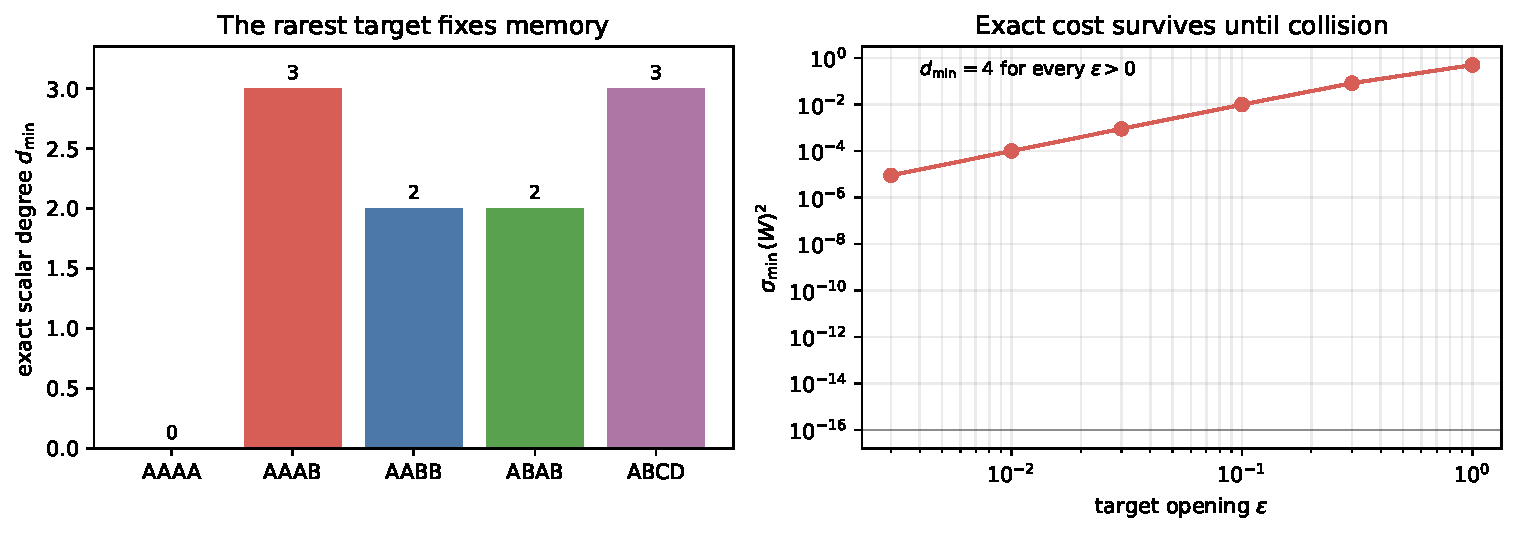
\includegraphics[width=0.98\linewidth]{figures/unified_routing_table_memory.pdf}
\caption{Left: the scalar occupancy law is not ordered by switch count.
Right: the direct-sum margin closes continuously in the collision family,
while the exact degree stays four for every positive opening and drops only
at the singular endpoint.  Curves use exact constructions, not fitted
asymptotics.}
\label{fig:summary}
\end{figure}

\section{Executable audit}

The numerical layer is deliberately subordinate to the proof.  The
producer samples dense nonorthogonal target frames, forms a left inverse,
checks all dual block isolations, assembles $F_0$, and verifies strict
positivity of $F_0^*F_0$ on a boundary grid.  For $k=1$ it independently
computes the outer scalar spectral factor and checks the normalized
rational-inner column.  Block trials with $k=2,3$ audit the matrix precursor
and target ranges without pretending that floating-point factorization
proves the matrix Fej\'er--Riesz theorem.

The frozen campaign has 512 scalar and 256 block tables plus six collision
openings.  The largest dual-isolation residual is
$1.17\times10^{-11}$; the largest target-projector error is
$8.72\times10^{-11}$; the largest wrong dual minor is
$1.79\times10^{-11}$; and the smallest sampled density eigenvalue is
$7.82\times10^{-9}$.  In the scalar spectral-factor replay, the largest
relative factor residual is $2.37\times10^{-8}$ and the largest boundary
isometry residual is $1.78\times10^{-5}$.  The latter is attained in an
ill-conditioned fixture and is reported rather than hidden.

An independent verifier imports no producer code.  It recomputes the
rarest-occupancy examples and a fresh direct-sum dual fixture, validates the
canonical JSON digest, and enforces every numerical tolerance.  Both
programs fail closed.

\begin{table}[t]
\centering\small
\caption{Theorem-to-artifact map.  Paths are relative to the immutable
release printed below.}
\label{tab:artifacts}
\begin{tabular}{@{}L{0.32\linewidth}L{0.60\linewidth}@{}}\toprule
Claim & Executable witness\\\midrule
Dual detectors and spectral compiler & \path{research/unified_routing_table_certificate.py}\\
Exact detector-rank incidence fixtures & \path{research/detector_rank_hierarchy_certificate.py}\\
Frozen campaign and digest & \path{results/unified_routing_table_memory/certificate.json}\\
Independent fail-closed replays & \path{verification/verify_unified_routing_table_memory.py},
\path{verification/verify_detector_rank_hierarchy.py}\\
Collision and occupancy figure & \path{paper_unified_routing_table_memory/figures/unified_routing_table_memory.pdf}\\
Paper source and submission record & \path{paper_unified_routing_table_memory/}\\
\bottomrule\end{tabular}
\end{table}

\section{Positioning, limits, and claims}

Minimal rational interpolation, boundary matrix Schur interpolation, and
McMillan-degree analysis have an extensive theory
\cite{AntoulasEtAl1990,BallKim1994,BolotnikovDym2006,GombaniMichaletzky2007}.
Matrix all-pass design by subspace Nevanlinna--Pick interpolation can also
prescribe unitary data and group-delay blocks \cite{BharathEtAl2023}.
Matrix Fej\'er--Riesz factorization and rectangular lossless completion are
classical \cite{DritschelRovnyak2009,AlpayJorgensenLewkowicz2016}.

The new results are not any one of those ingredients.  They are the exact
direct-sum occupancy identity \eqref{eq:master}, including its dual-minor
necessity and target-weighted matrix spectral compiler, and the
detector-rank hierarchy \eqref{eq:detector-rank-bound} on arbitrary
equal-rank arrangements.  A targeted search of the primary literature
through 11 August 2026 did not locate the occupancy formula, the statement
that least occupancy is a complete generic state statistic, or the weighted
rank-deficiency bound in this routing form.  This supports priority claims
for these precise eliminations, not for rational-inner interpolation,
Potapov factorization, or projective geometry in general.

\begin{limitation}[Exact comparison class]
The master theorem assumes distinct nodes, exact subspace data, equal target
rank, free endpoint gauges, rationality, and losslessness.  Repeated nodes
require confluent or jet interpolation.  Fixed frames turn phases into data.
Unequal ranks create a multiplicity-packing problem.  Active or lossy
architectures do not obey the inner-function zero and delay budgets.
\end{limitation}

\begin{limitation}[Singular geometry]
Outside direct-sum position, \cref{eq:sandwich,eq:detector-rank-bound} remain
valid but neither occupancy nor the detector-rank statistic alone need
determine degree.  The paper does not claim a complete equality formula for
every intersection lattice; the hierarchy captures all constant
determinantal detectors, while compatibility of their upper constructions
is a separate problem.
\end{limitation}

\begin{limitation}[Conditioning versus degree]
Exact McMillan degree is integer-valued and insensitive to node spacing on
the theorem's locus.  Realization coefficients and spectral-factor
conditioning are not.  Near node or target collisions, stable numerical
synthesis may require higher precision even though the exact degree is
unchanged.
\end{limitation}

The next mathematical frontier is therefore sharper than before: determine
when the detector-rank lower hierarchy is attainable and which families of
minors can share one state budget on a prescribed intersection lattice.  The
next physical frontier is a robust approximate law coupling node separation,
projector error, and allowed leakage.  Neither problem is concealed inside
the present exact claims.

\section{Conclusion}

A finite spectral routing table has a simple generic memory law and a
geometric singular lower theory.  Direct-sum geometry creates a dual
detector for every target; every absence consumes $k$ determinant zeros, so
the least visited target asks for the largest budget.  More generally, every
constant detector charges the occupancy-weighted rank deficiency
\[
                 \sum_a n_a\bigl(k-\rank(D_{\rm det}|_{Y_a})\bigr).
\]
A matrix Fej\'er--Riesz compiler shares exactly the direct-sum budget across
all detectors.  The equality
\[
                         d_{\min}=k(L-n_*)
\]
therefore unifies orthogonal fan-out, generic fan-out, and routing words,
while the detector hierarchy, collision family, and constructive three-line
lemma expose what survives on singular strata.  On the direct-sum locus the
same integer is at once a state count, a determinant-winding count, and the
optimal integrated Wigner--Smith action divided by $2\pi$.

\paragraph{Immutable reproducibility record.}
Full release URL (tag included):
\begin{center}\small
\url{https://github.com/lluiseriksson/finite-sample-spectral-certificates/releases/tag/v2.8-ai-vixra-submission}
\end{center}
The release records the exact target commit, PDF SHA-256, producer commands,
independent verifiers, and CI status.  Release v2.8 supersedes v2.7 as the
submission artifact of this same unified paper.  The three predecessor
preprints remain citable historical records, but the present article absorbs
their scientific scope rather than counting them as additional current
results.

\bibliographystyle{plain}
\bibliography{references}
\end{document}
